%! program = pdflatexmk

% Free Democracy Foundation Mobile Voting Threat Model Top-Level Document
% Copyright (C) 2024-25 Free & Fair
% Last Revision: 2025-03-19 Daniel M. Zimmerman

\documentclass[10pt,letterpaper]{article}

%%% PACKAGES
\usepackage[letterpaper, total={7.5in, 9in}]{geometry}
\usepackage[in]{fullpage}
\usepackage{tabularray}
\usepackage[pdftex,bookmarks,colorlinks,breaklinks]{hyperref}
\usepackage{amsmath}
\usepackage{amssymb}
\usepackage{listings}
\usepackage{verbatim}
\usepackage{lmodern}
\usepackage[T1]{fontenc}
\setlength {\marginparwidth}{2cm}
\usepackage{todonotes}
\usepackage{enumitem}
\usepackage[backend=biber, style=numeric, sorting=nyt]{biblatex}
\usepackage{etoolbox}

%%% Draft Boolean: controls the draft watermark and the version
%%% string at the top of page 1

\newbool{draft}
\setbool{draft}{false} %%% CHANGE THIS FOR DRAFT

%%% Draft Watermark
\ifbool{draft}{\usepackage[]{draftwatermark}}{}

\addbibresource{references.bib}
\parindent 0pt
\setlength{\parskip}{10pt plus 1pt minus 1pt}

\usepackage{tocloft}
\setlength\cftparskip{2pt}

\renewcommand{\subsectionautorefname}{section}
\renewcommand{\subsubsectionautorefname}{section}

% Don't use URL dates for non-online items
\AtEveryBibitem{\ifentrytype{online}{}{\clearfield{url}\clearfield{urlyear}}}

% by default, don't put headings on tables
\DefTblrTemplate{firsthead, middlehead,lasthead}{default}{}

% detect Overleaf using the job name
\ifnum\pdfstrcmp{\jobname}{output}=0
% "Dark Mode" for Overleaf ------
\usepackage{xcolor}
\pagecolor[rgb]{0,0,0} %black
\color[rgb]{0.7,0.7,0.7} %grey
\hypersetup{linkcolor=yellow,citecolor=yellow,filecolor=white,urlcolor=yellow}
% ----------------------
\else
\hypersetup{linkcolor=blue,citecolor=blue,filecolor=black,urlcolor=blue}
% nothing else to do in non-Overleaf case for now; perhaps
% this will automatically trigger export of tables later
\fi

%%% BEGIN DOCUMENT
\begin{document}

\begin{center}
{\Large \textbf{E2E-VIV Cryptographic Core Threat Model}}
\end{center}
\vspace{-6pt}

% note: until we finalize the details of the protocol, we aren't going to call this threat model "1.0"
\notbool{draft}{\textit{Version 0.9}}{\textit{DRAFT---NOT FOR EXTERNAL DISTRIBUTION}} \hspace{\fill} \textit{April 2025}

\vspace{-12pt}

\rule{\textwidth}{1pt}

\tableofcontents

\section*{Introduction}
\label{sec:intro}
\addcontentsline{toc}{section}{\nameref{sec:intro}}

This is the threat model for the family of E2E-VIV systems being developed for the \href{https://freedemocracyfoundation.org/}{Free Democracy Foundation} \href{https://mobilevoting.org/}{mobile voting project}. This document describes the principals (subsystems, actors, and assets) involved, the system entry/exit points, trust zones, and trust levels, the data flows within the system, and the identified threats, risks, and mitigations.

As we are developing the cryptographic core to be used in E2E-VIV systems, rather than an entire actual E2E-VIV system for deployment, multiple aspects of a full system (such as voter registration, voter requests for digital absentee ballots, etc.)~are either not represented, or only represented as high-level abstractions, in this threat model. Despite this, for brevity, we refer to the system we are developing as the ``E2E-VIV system'' throughout the remainder of this document.

This protocol's overall ``shape'' is based upon earlier extensive work funded by the Mobile Voting Project. In particular, earlier projects worked extensively with U.S. election officials to understand their needs and goals, particularly with respect to the use of existing election management and tabulation systems, and the need for paper ballot records for all early ballots, digitally cast or otherwise.

The core constraint of the remote/Internet voting-augmented election workflow adopted through previous projects is that \emph{paper ballots must be printed for all cast digital ballots so that existing paper ballot tabulators can be used for tabulation}. We do not make any assertions or assumptions about audits, risk-limiting or otherwise, of paper ballots produced by such a system.

This scope means that there are a number of weaknesses and attacks that we \emph{explicitly do not mitigate} as a part of the protocol and its implementation. Those attacks and weaknesses must be mitigated by the design, architecture, engineering, assurance, deployment, and management of any product that uses this cryptographic protocol/library. The relevant mitigations (\hyperlink{M8}{M8} through \hyperlink{M12}{M12} in the model) have names that start with ``Cybersecurity'', and include attacks and weaknesses such as malware on voter devices.

We encourage you to use the issue and security report functionality of our \href{https://github.com/FreeAndFair/MobileVotingCoreCryptography}{public GitHub repository} to report any errors you find within this threat model and to make suggestions that you think might be helpful for future versions. If you do so, note that the E2E-VIV protocol is still under active development and that certain aspects of it, particularly the submission scheme, are still subject to change.

\section{Related Work}
\label{sec:related_work}

Our bibliography for threat modeling and security engineering is extensive. Threat modeling as a discipline is described or used in Government standards~\cite{JointTaskForceTransformationInitiativeGuideconductingrisk2012} and several books which either focus exclusively on threat modeling, or are general-purpose security engineering books that contain chapters on threat modeling~\cite{ShostackThreatmodelingdesigning2014,TarandachColesThreatModeling2020,SwiderskiThreatModeling2004,AndersonSecurityEngineeringGuide2020,DeogunSecureDesign2019,WoodyCyberSecurityEngineering2016,BishopComputerSecurityArt2018,IdreesModelSystemAdversary2014}.

Since this project focuses on a family of cryptographic protocols for realizing End-to-End Verifiable Internet Voting and their dependent algorithms, a number of cryptography textbooks are also foundational~\cite{FergusonCryptographyEngineeringDesign2010,DanBonehGraduateCourseApplied2023,KatzIntroductionModernCryptography2007}.

We have also reviewed official documents (statutes, standards, rules, etc.) produced by other governments~\cite{AustralianSignalsDirectorateEtAlChoosingSecure,EuroparatStandardsEvoting2018} and government working groups constructed to study the idea of Internet voting, or reflect upon the roll-out of (successful or not) Internet voting platforms and services in other countries and settings~\cite{ElectoralCouncilofAustralia&NewZealandElevenEssential2017,BruterEtAlStudyEVoting2023,BagnatoRecommendationCMREC201752022,AppelCACVoteAnother2024}. We are particularly attentive to U.S.~Government cybersecurity strategy and implementation~\cite{TheWhiteHouseNationalCybersecurity2023,TheWhiteHouseNationalCybersecurity2023a,TheWhiteHouseNationalCybersecurity2024}.

Scientific critiques of deployed Internet voting platforms are a rich source of information~\cite{KiniryFormallyCountingElectronic2007,KiniryKOARemoteVoting2007,WolchokAttackingWashingtonDC2012,TeagueProblemsiVoteInternet2012,HaldermanNewSouthWales2015a,SpringallSecurityAnalysisEstonian2014}. This includes platforms that were previously evaluated by the Tusk Montgomery Philanthropies Foundation, such as Voatz and Democracy Live~\cite{TrailofBitsVoatzSecurityAssessment2020,TrailofBitsVoatzSecurityAssessment2020a,SpecterEtAlBallotBusted2020,SpecterSecurityAnalysisDemocracy2021}.

Additional key framing documents include publications from Verified Voting~\cite{VerifiedVotingCastingVotesSafely2023,VerifiedVotingInternet} and the National Academies of Sciences, Engineering, and Medicine~\cite{CommitteeontheFutureofVoting:AccessibleReliableVerifiableTechnologySecuringVoteProtecting2018}.

We position all of our language and analysis within the framing of several overarching documents that describe the challenges and opportunities of digital/computer-based voting, whether over the Internet or otherwise~\cite{Dzieduszycka-SuinatFutureVotingEndtoEnd2015a,U.S.ElectionAssistanceCommissionVoluntaryVoting2021}.

Our approach is based upon years of work with U.S.~Government agencies on the design, implementation, assurance, and certification of national security systems and nationally critical infrastructure. Our methodology is grounded in related work~\cite{PeterLoscoccoAssumptionDrivenDesignStrategy}, and our implementation strategy, such as our use of safe programming languages and formal methods as a means of assurance is grounded in new U.S.~Government recommendations, standards, and requirements~\cite{OfficeoftheNationalCyberDirector:TheWhiteHouseBackBuilding2024,UnitedStatesCybersecurityandInfrastructureSecurityAgencyEtAlCaseMemory2023,DefenseScienceBoardTaskForceUndersecretaryofDefenseforResearchandEngineeringFutureCyberWarfighting2024,DefenseScienceBoardTaskForceUndersecretaryofDefenseforResearchandEngineeringSecureElectronicProcessing2025,DefenseScienceBoardTaskForceUndersecretaryofDefenseforResearchandEngineeringTestEvaluationTE2024,TheWhiteHouseSummary2023Request2024,CybersecurityandInfrastructureSecurityAgencyCISAEtAlShiftingBalance}.

Because traditional threat models are created \emph{manually} through teamwork, wisdom, and peer-review, one can \emph{never} be sure that a threat model is complete with respect to all current or future possible adversaries, attacks, threats, or weaknesses. Only by using the collective wisdom of past analyses and the aggregate, long-term lessons learned from other experimental or deployed similar systems (both successes and, especially, failures) can we have confidence in a even a semi-formal threat model, like we have created here.

Moreover, identifying, implementing, and assuring mitigations requires design choices that balance security against other non-behavioral system properties such as implementation complexity, system performance, latency, network overhead, etc.

\pagebreak
\section{Subsystems}

The E2E-VIV system is comprised of the following subsystems:\footnote{We are still in the process of formally specifying the cryptographic protocol; as a result of that specification this list may change, at which point the remainder of the threat model will be updated accordingly.}

\begin{itemize}

    \item \textbf{Voting Application}: the client-side mobile application used by a voter to authenticate to the system, make choices on a ballot, and cast or check a voted ballot

    \item \textbf{Voting Device}: the client-side mobile device on which the Voting Application runs

    \item \textbf{Authentication Service}: a service used by the voting application server to authenticate voters' identities, so that their eligibility to vote in a specific election can be determined; in any given instantiation of the system, this service may be provided by multiple external identity service providers

    \item \textbf{Public Bulletin Board}: the canonical, publicly-readable, append-only view of election information; can only be appended to by the \textbf{Digital Ballot Box}

    \item \textbf{Digital Ballot Box}: the system that stores submitted digital ballots, which can be used for ballot checks and, post-election, for tallies; this system determines when information can be appended to the \textbf{Public Bulletin Board}

    \item \textbf{Trustee Application}: the client-side application with which trustees interact in order to generate their private key shares and open/close the election, and perform partial ballot decryption in a mix-net configuration; this application runs on a dedicated device, one of which exists for each trustee, and must not be directly connected to the Internet at any point during the system's lifetime

    \item \textbf{Trustee Administration Server}: the system that orchestrates the generation of cryptographic keys (and associated threshold secret sharing) related to the election before the election begins, and ballot decryption or homomorphic tallying once the election is complete; must not be connected to the Internet at any point during the system's lifetime

    \item \textbf{Election Administration Server}: the system(s) used by election officials to handle election definition and administration functions, including voter authorization (based on registration records), ballot definitions, election start/end times, etc.;~note that we treat this as a single abstract subsystem in sequence diagrams for simplicity, though in a concrete implementation the election administrator interacts with it using the \textbf{Election Administrator Application}

    \item \textbf{Election Administrator Application}: the system in an election office used by election officials to communicate with the \textbf{Election Administration Server} and import/export data using \textbf{Election Administrator Storage}

    \item \textbf{Ballot Checking Application}: a client-side (web-based or mobile) application used by a voter to perform ballot checks; there may be multiple independent ballot check applications in any instantiation of the system

    \item \textbf{Ballot Printer}: a printer that produces \textbf{Paper Ballots} from \textbf{Cast Digital Ballot Plaintexts}, only part of the system in variants that perform mix-net decryption and print ballots for physical tally; most likely implemented by a standard printer combined with a software component on the \textbf{Trustee Administration Server} that converts \textbf{Cast Digital Ballot Plaintexts} to an appropriate digital format

\end{itemize}

\pagebreak
\section{Actors}

The following actors\footnote{Some of the subsystems above (e.g., \textbf{Voting Application}) may also exhibit actor-like behavior, as they can be corrupted (e.g., by malware on a \textbf{Voter}'s device changing the behavior of the \textbf{Voting Appication} to abuse the server APIs), but we do not list them separately here.} participate in the operation of the E2E-VIV system:

\begin{itemize}

    \item \textbf{Voters}: people who use the system to cast ballots and optionally check that they have been properly recorded

    \item \textbf{Election Administrator}: a person who facilitates protocols and procedures, provides the election definition, and publishes the election results; this is a single actor in the system even though its responsibilities may be shared among multiple people in a given system instantiation

    \item \textbf{Trustees}: people who are jointly responsible for maintaining the privacy of the votes, and for performing/facilitating the vote tally, by keeping custody of election key shares

    \item \textbf{Verifiers}: people that evaluate the election records to confirm an election's integrity; verifiers may use any means at their disposal (verification programs, pencil and paper, etc.)~to verify the results based on public information available from the \textbf{Digital Ballot Box}, and they have no direct role in the election

\end{itemize}

\section{Assets}

The E2E-VIV system has the following assets:

\begin{itemize}

    \item \textbf{Election Administrator Credentials}: used to perform election administration functions

    \item \textbf{Trustee Private Key Shares}: shares of the election's private key held by individual \textbf{Trustees}; used to partially decrypt or homomorphically tally \textbf{Digital Ballot Cryptograms} exported from the \textbf{Digital Ballot Box}

    \item \textbf{Election Public Key}: the public key corresponding to the complete set of \textbf{Trustee Private Key Shares}; used in the creation of \textbf{Digital Ballot Cryptograms}

    \item \textbf{Digital Ballot Box API Credentials}: used to write ballot/election information to the \textbf{Digital Ballot Box}

    \item \textbf{Voter Roster}: a list of \textbf{Voter}s who are eligible to participate in a particular election

    \item \textbf{Election Manifest}: the definition of an election, including all contests and selectable options, contest selection limits, ballot styles, and appropriate/necessary metadata about the election's timing, software versions, etc.; serves as a common view of the election shared by all actors, publicly visible in the \textbf{Digital Ballot Box}

    \item \textbf{Digital Ballot Cryptograms}: encrypted digital representations of ballots that have been submitted to the \textbf{Digital Ballot Box} by \textbf{Voters} using the \textbf{Voting Application}; these may end up being either cast or checked

    \item \textbf{Cast Digital Ballot Plaintexts}: decrypted digital representations of ballots that have been cast by \textbf{Voter}s using the \textbf{Voting Application}; these should only ever exist within the \textbf{Trustee Administration Server}'s trust zone

    \item \textbf{Checked Digital Ballot Plaintexts}: decrypted digital representations of ballots that have been checked by \textbf{Voter}s using the \textbf{Ballot Check Appplication}; these are publicly available in the \textbf{Digital Ballot Box}

    \item \textbf{Printable Cast Ballots}: printable files that represent ballots cast in the election, which enable traditional optical-scan or hand tallying of paper ballots in some mix-net based system configurations

    \item \textbf{Trustee Storage}: a piece of hardware for each trustee that stores their \textbf{Trustee Private Key Share}; this will most likely be a fresh, ecrypted USB storage device, and must never be attached to an Internet-connected device during the system's lifetime

    \item \textbf{Election Administrator Storage}: a piece of hardware for the election administrator that is used to convey information between the \textbf{Election Administration Server}/\textbf{Digital Ballot Box} and the \textbf{Trustee Administration Server} (across an air gap); this will most likely be a fresh, encrypted USB storage device

\end{itemize}

\section{Entry/Exit Points}

The E2E-VIV system has the following entry and exit points (data transfer between the air-gapped network and the rest of the system is considered an entry/exit for this purpose):

\begin{itemize}

    \item \textbf{Digital Ballot Box}: an exit point for \textbf{Digital Ballot Cryptograms} and  \textbf{Checked Digital Ballot Plaintexts}

    \item \textbf{Trustee Application}: an entry and exit point for \textbf{Trustee Private Key Shares} (the trustees need to enter them back into the system in order to perform tallying/decryption)

    \item \textbf{Election Administrator Application}: the entry point for election configuration, voter eligibility determinations, and other election administration parameters; an entry and exit point for the \textbf{Election Manifest}; and an exit point for \textbf{Cast Digital Ballot Cryptograms} (by writing them to \textbf{Election Administrator Storage})

    \item \textbf{Trustee Administration Server}: an entry and exit point for the \textbf{Election Manifest}, the exit point for the \textbf{Election Public Key}, an entry point for \textbf{Cast Digital Ballot Cryptograms}, and, in configurations where ballots are decrypted and printed, the exit point for \textbf{Printable Cast Ballots}

\end{itemize}

\section{Trust Zones}

The E2E-VIV system has the following trust zones:

\begin{itemize}

    \item \textbf{Air-Gapped Network}: a network sequestered from the global Internet and all other trust zones of the system that houses the \textbf{Trustee Application} and \textbf{Trustee Administration Server}; entry to/exit from this zone is exclusively by physical devices (USB storage, paper, direct keyboard input of physical randomness such as dice roll results, etc.)

    \item \textbf{Election Office Network}: the network that houses the system exit point used to export data for transfer to the \textbf{Air-Gapped Network}; this network is physically located in an election office

    \item \textbf{Election Administration Network}: the network that houses the \textbf{Election Administration Server}, \textbf{Digital Ballot Box}, and \textbf{Public Bulletin Board}; this network may be connected to the \textbf{Internet}, and may be located either in the cloud or in an election office

    \item \textbf{Internet}: the Internet, to which many subsystems (e.g., \textbf{Voting Application}) are directly connected and which connects all trust zones except the \textbf{Air-Gapped Network}

\end{itemize}

\section{Trust Levels}
The E2E-VIV system has the following trust levels:

\begin{itemize}

    \item \textbf{Election Administrator}: full, physical access to the \textbf{Election Administration Server} (or to the \textbf{Election Administrator Application} that has full access to the \textbf{Election Administration Server}, if the latter is in the cloud) and \textbf{Trustee Application Server} for election configuration and protocol/procedure facilitation

    \item \textbf{Trustee}: able to physically access the device hosting a single \textbf{Trustee Application} (and thus to hold a single \textbf{Trustee Private Key Share}), no access to any other subsystem beyond what is available at the \textbf{Public} trust level

    \item \textbf{Voter}: able to use the \textbf{Voting Application} and any number of \textbf{Ballot Check Applications}, no access to any other subsystems beyond what is available at the \textbf{Public} trust level; note that technically, anybody can run and interact with either of these applications (or, for that matter, attempt to use the APIs of any of the servers connected to the \textbf{Internet}), but only a registered \textbf{Voter} can actually cast a vote or get sufficient information from the \textbf{Voting Application} to check a vote

    \item \textbf{Public}: able to read the public information from the \textbf{Digital Ballot Box}; able to access any Internet-accessible endpoint of the system in any allowed uncredentialed way

Note that some individuals, notably \textbf{Election Administrators}, have multiple simultaneous trust levels (as they are both administrators and \textbf{Voters}).

\end{itemize}

\pagebreak
\section{Data Flow Diagrams}

In this section, we present data flow diagrams that illustrate, at a high level, the flow of data among principals and trust zones within the system. We first show an overall diagram of the entire system, then specific protocol data flows related to voter interactions (authentication, voting, checking and casting ballots) and trustee interactions (generating the election's keys before the election begins, handling cast ballots after the election is concluded).

These diagrams are \emph{not} a specification of the (distributed, cryptographic) algorithm that sits underneath our protocol. The precise, formal specification of that algorithm is underway now, using the Tamarin and ProVerif protocol specification and verification tools~\cite{ChevalSAPICprotocolverifiers2022,MeierTAMARINProverSymbolic2013,BlanchetModelingVerifyingSecurity2016}.\footnote{As with the list of subsystems, these diagrams will evolve as we complete our precise specification of the cryptographic protocol.}

\subsection{Overall Data Flow and Trust Zones}

This diagram is an overview of the system's trust zones and principals, and the dataflows that exist among them. It does not contain details about the dataflow contents or sequencing, and exists solely to show where and how the trust zones are connected to each other during system execution.

Note that the \textbf{Voter} interacts with the \textbf{Voting Application}, \textbf{Authentication Service}, and \textbf{Ballot Check Application} using at least one, but possibly multiple, computing devices. It is expected that the \textbf{Voting Application} is a native application on an iOS or Android device that supports biometrics, and that the \textbf{Ballot Check Application} is either a native application or a web application. The \textbf{Authentication Service} could be provided by any of a number of identity authentication providers, and is deliberately left underspecified.

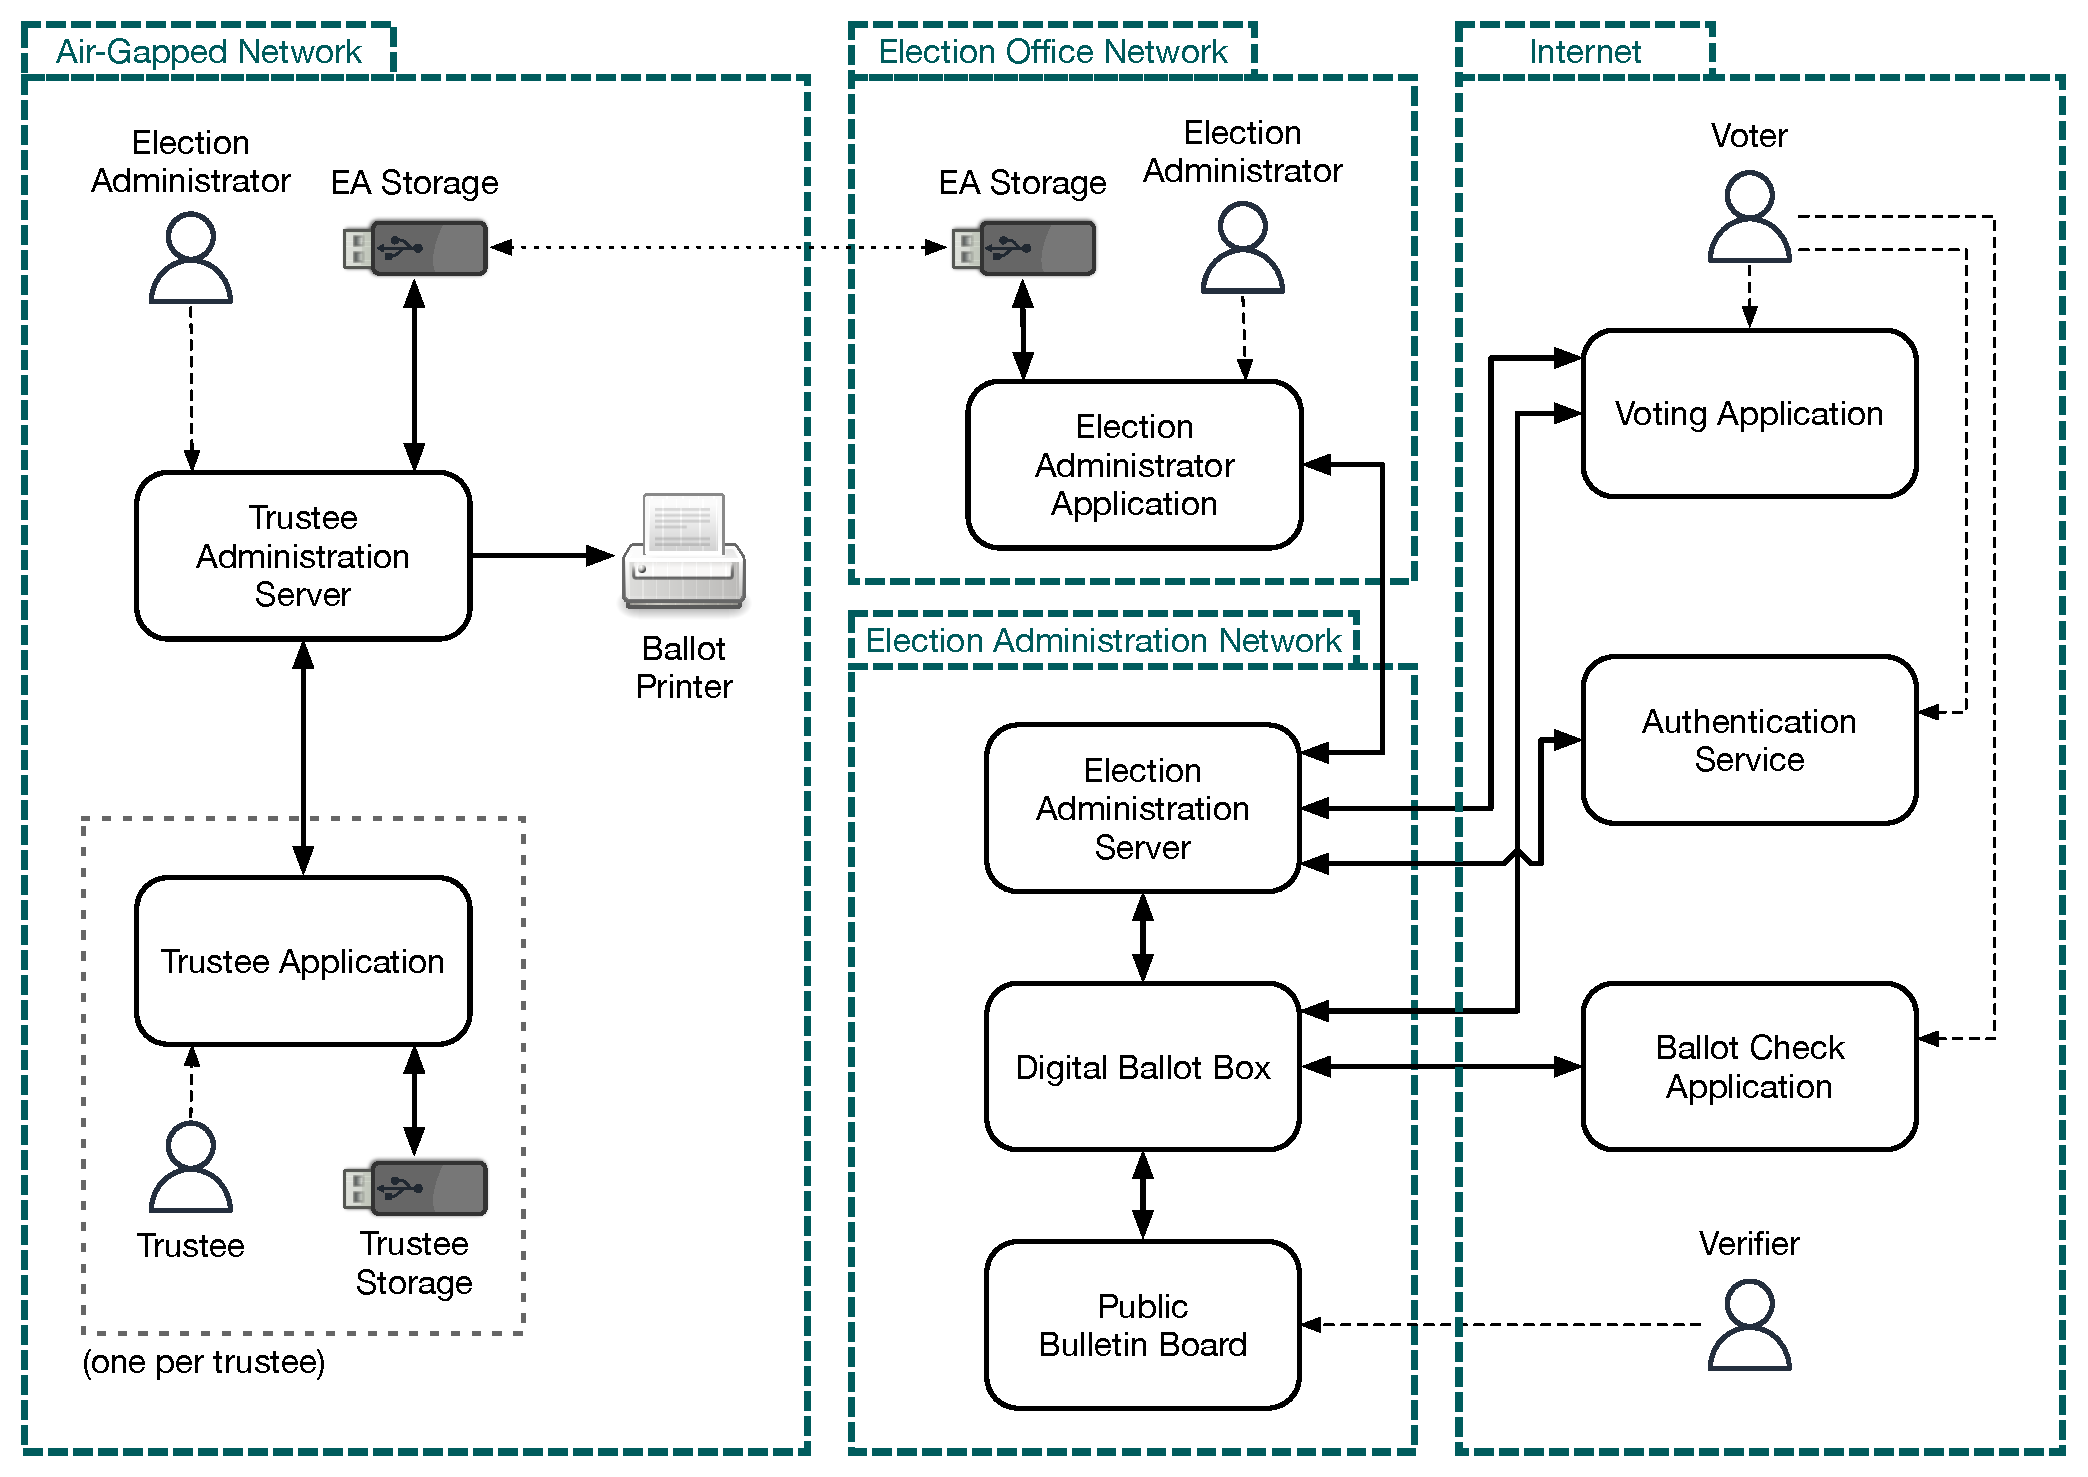
\includegraphics[width=\textwidth]{diagrams/system-overview.pdf}

\pagebreak
\subsection{Voter Authentication and Choice Sequence}

This is the first part of a \textbf{Voter}'s interaction with the system, encompassing authentication and making ballot choices. Once the \textbf{Voter} makes their choices (assuming they authenticate successfully and have an election to participate in), they move on to perform the \hyperlink{voter-ballot-check-sequence}{Voter Ballot Check Sequence} zero or more times before performing the \hyperlink{voter-ballot-cast-sequence}{Voter Ballot Cast Sequence} to conclude their interaction with the system.

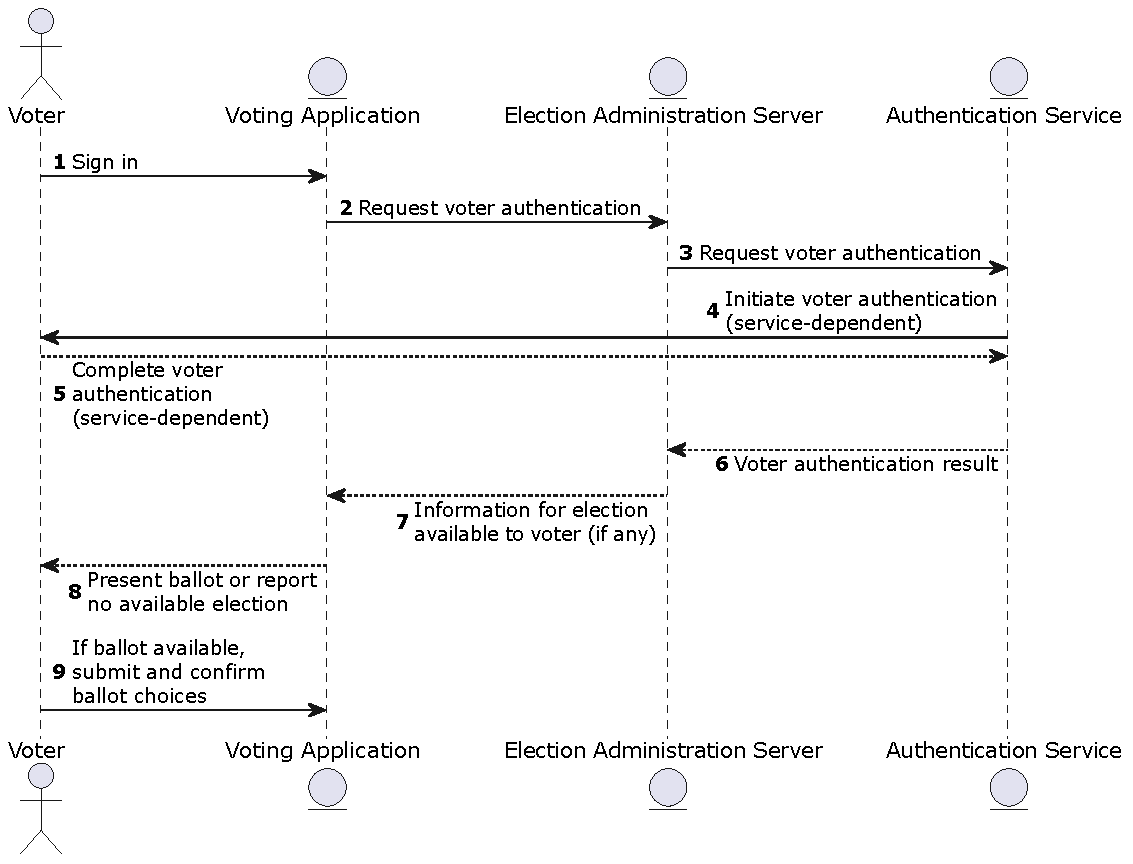
\includegraphics[width=\textwidth]{diagrams/seq-voter-auth-choice.pdf}

\pagebreak
\subsection{Voter Ballot Check Sequence}
\hypertarget{voter-ballot-check-sequence}{}

This part of a \textbf{Voter}'s interaction with the system covers the ballot check functionality.

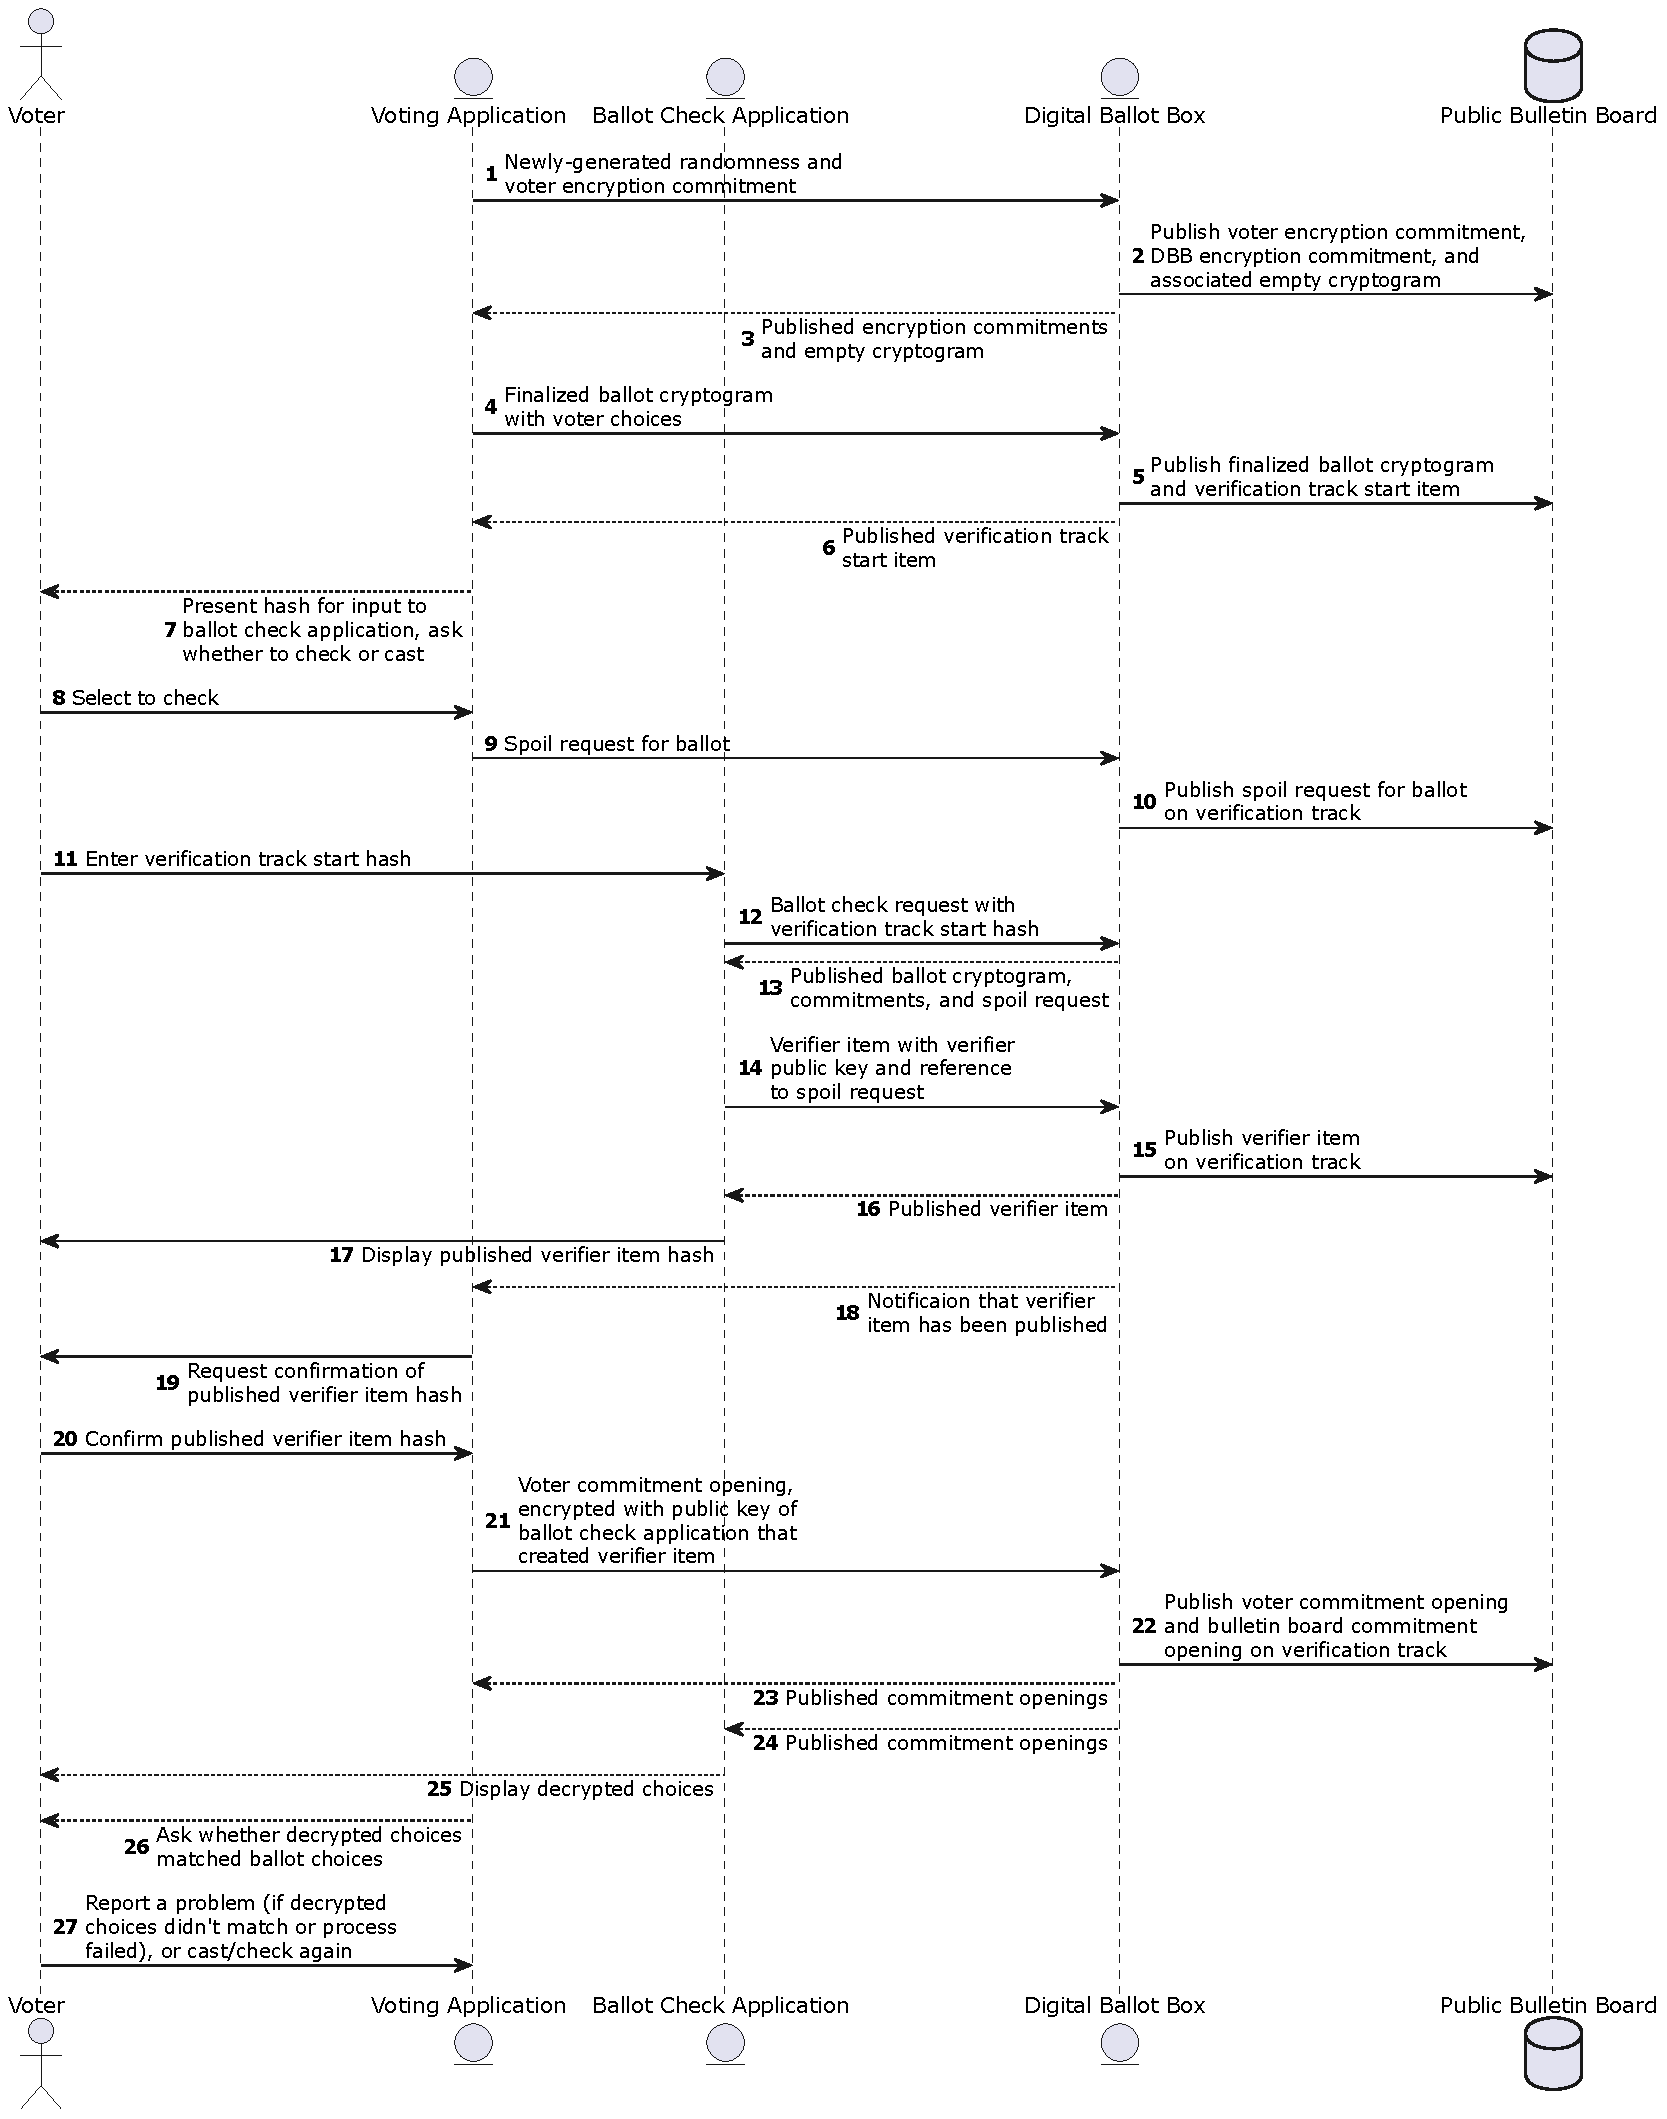
\includegraphics[width=0.95\textwidth]{diagrams/seq-voter-ballot-check.pdf}

\pagebreak
\subsection{Voter Ballot Cast Sequence}
\hypertarget{voter-ballot-cast-sequence}{}

This part of a \textbf{Voter}'s interaction with the system covers the ballot cast functionality.

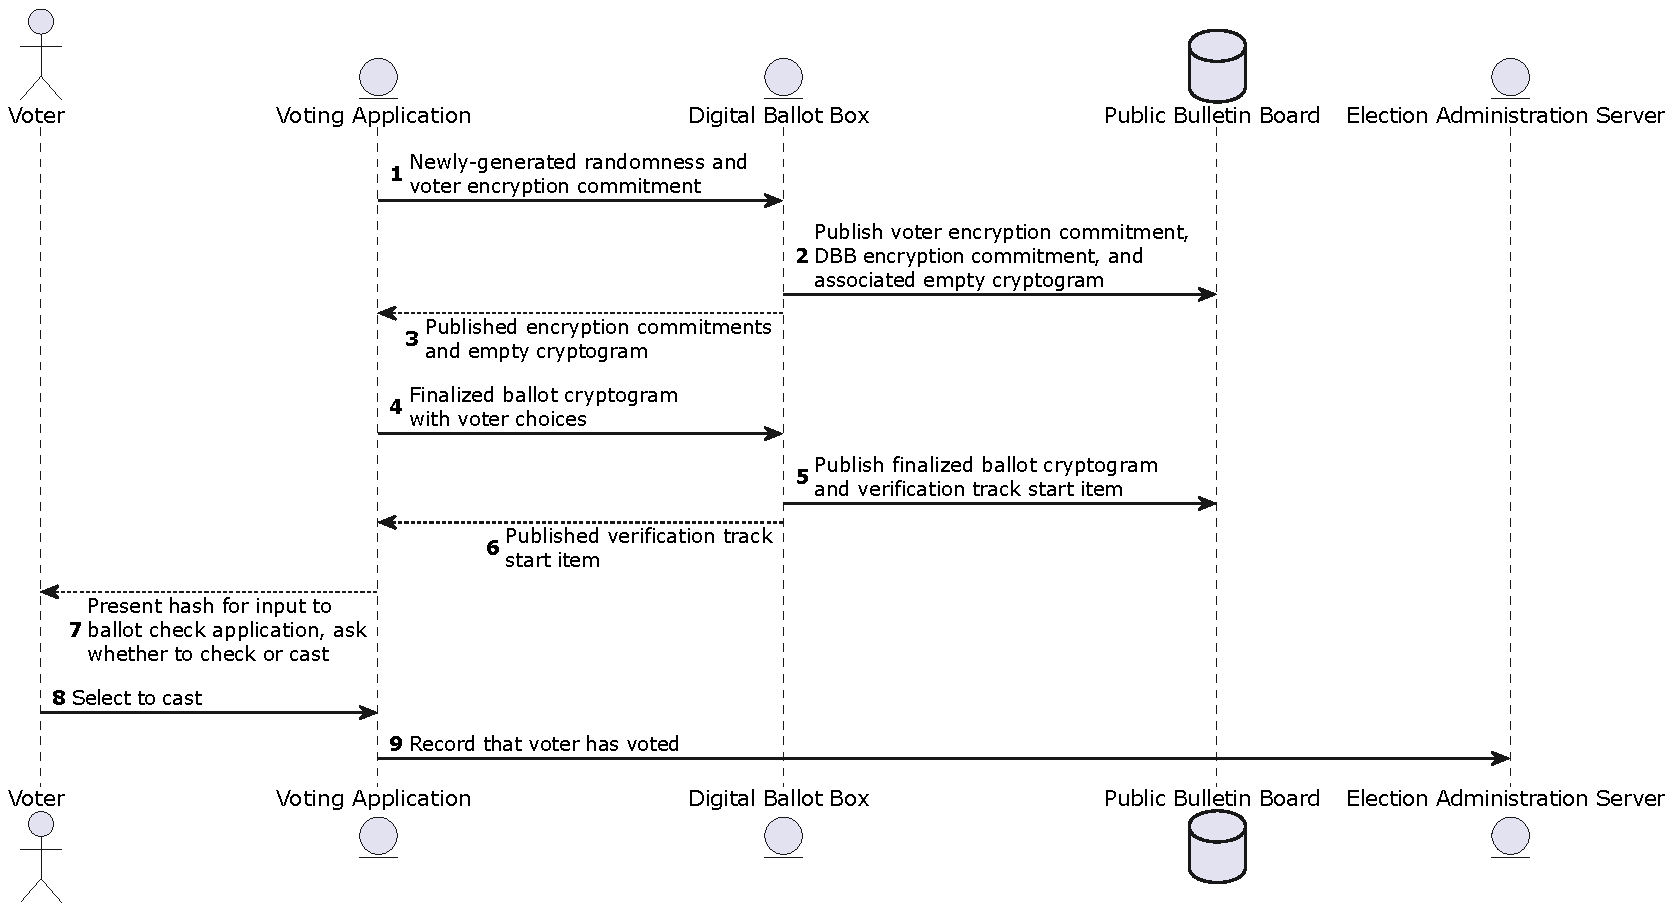
\includegraphics[width=\textwidth]{diagrams/seq-voter-ballot-cast.pdf}

\pagebreak
\subsection{Trustee Key Generation Sequence}

This part of a \textbf{Trustee}'s interaction with the system covers key generation. There is a separate \textbf{Trustee Application} (running on its own separate machine) and \textbf{Trustee Storage} device for each \textbf{Trustee}. The \textbf{Election Administrator} starts the process by loading data from the \textbf{Election Administration Server} (either directly or via the \textbf{Election Administrator Application}, which is not depicted in the sequence diagram) into the \textbf{Trustee Administration Server} via the \textbf{Election Administrator Storage} device, and the process concludes when the resulting \textbf{Election Public Key} has been written to the \textbf{Election Administrator Storage} device and all \textbf{Trustee Private Key Shares} have been written to their corresponding \textbf{Trustee Storage} devices.

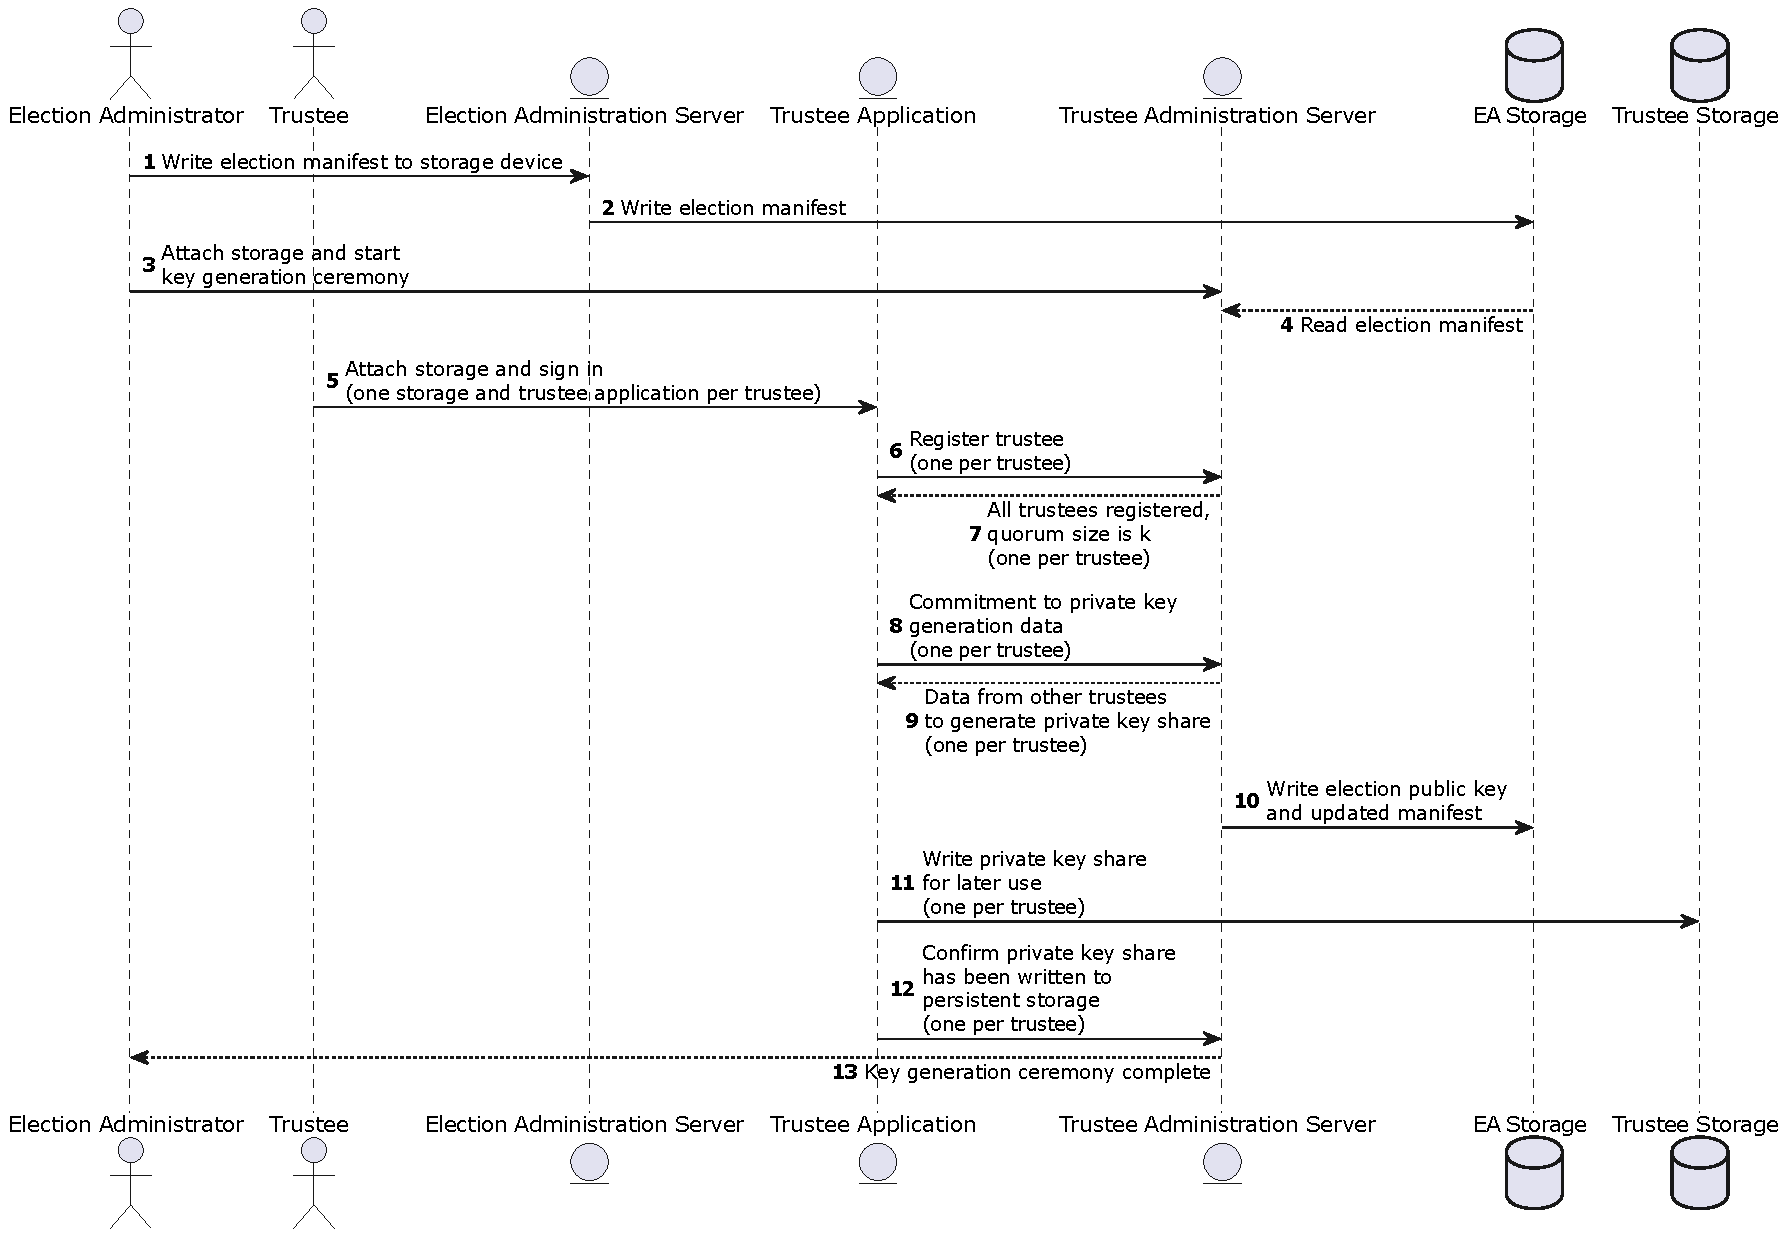
\includegraphics[width=\textwidth]{diagrams/seq-trustee-keygen.pdf}

\pagebreak
\subsection{Mix-Net Ballot Decryption/Printing Sequence}

This part of the \textbf{Election Administrator} and \textbf{Trustee} interaction with the system covers ballot decryption and printing. The \textbf{Election Administrator} starts the process by loading data from the \textbf{Digital Ballot Box} (either directly using the \textbf{Election Administration Server} or via the \textbf{Election Administrator Application}, which is not depicted in the sequence diagram) into the \textbf{Trustee Administration Server} via the \textbf{Election Administrator Storage} device. Once a sufficient quorum of \textbf{Trustees} sign in to their respective \textbf{Trustee Applications}, providing their private key shares from their \textbf{Trustee Storage} devices, the mixing and decryption is carried out by each trustee in sequence (that is, steps 11 and 12 are carried out by one trustee at a time, in some sequence, with each available trustee participating exactly once). Once all trustees have performed their mixes and partial decryptions, the ballots are printed for later tallying.

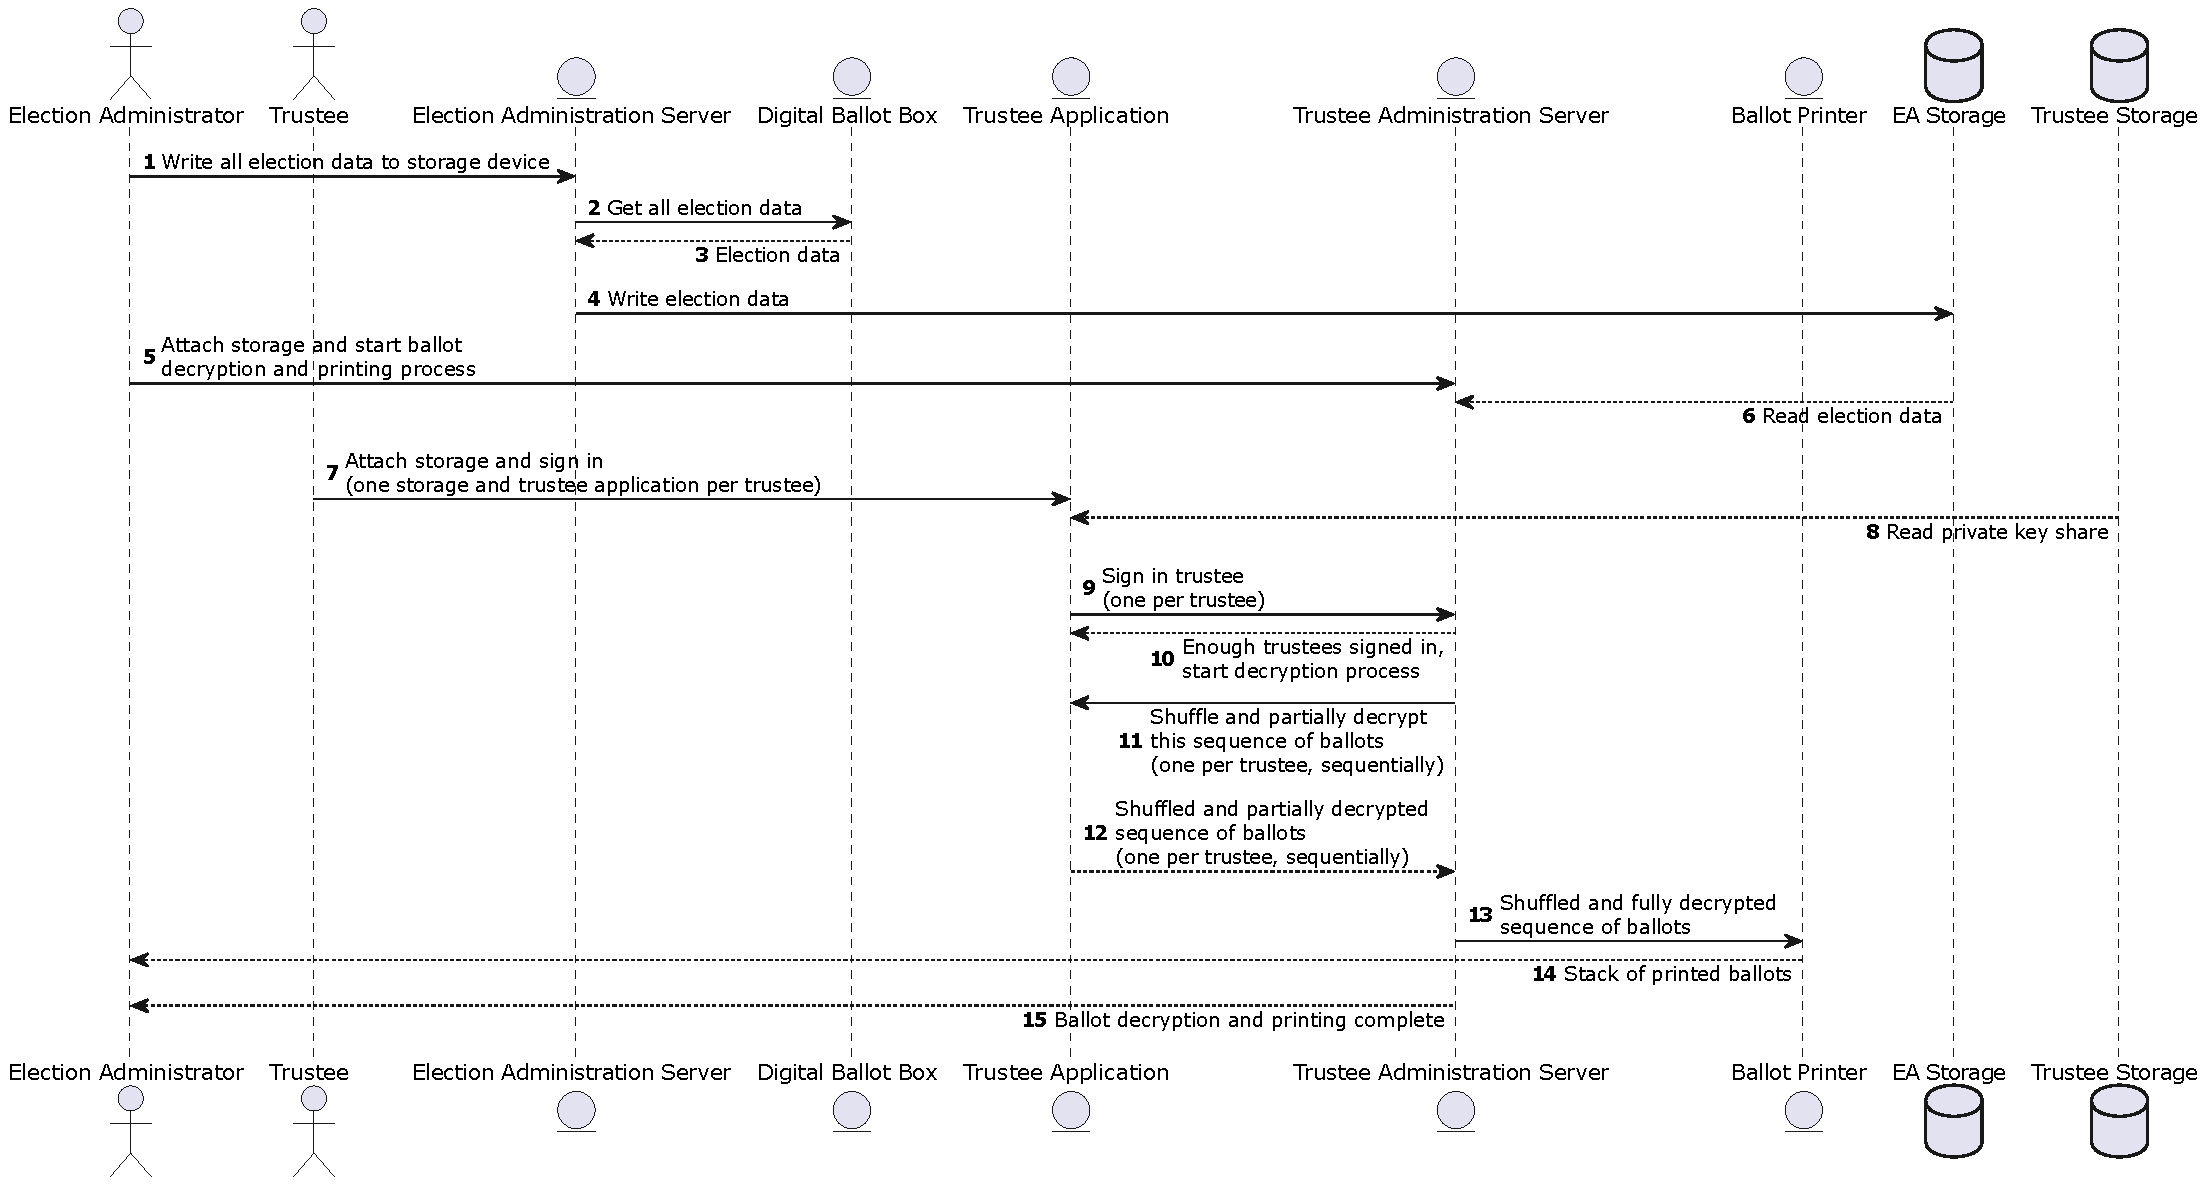
\includegraphics[width=\textwidth]{diagrams/seq-mix-net-decryption.pdf}

\pagebreak
\subsection{Homomorphic Ballot Tally Sequence}

This part of the \textbf{Election Administrator} and \textbf{Trustee} interaction with the system covers homomorphic tally of ballots. The \textbf{Election Administrator} starts the process by loading data (either directly using the \textbf{Election Administration Server} or via the \textbf{Election Administrator Application}, which is not depicted in the sequence diagram) from the \textbf{Digital Ballot Box} into the \textbf{Trustee Administration Server} via the \textbf{Election Administrator Storage} device. Once a sufficient quorum of \textbf{Trustees} sign into their respective \textbf{Trustee Applications}, providing their private key shares from their \textbf{Trustee Storage} devices, the homomorphic tally is computed, partially decrypted by each trustee in sequence (that is, steps 11 and 12 are carried out by one trustee at a time, in some sequence, with each available trustee participating exactly once), and written to the \textbf{Election Administrator Storage}.

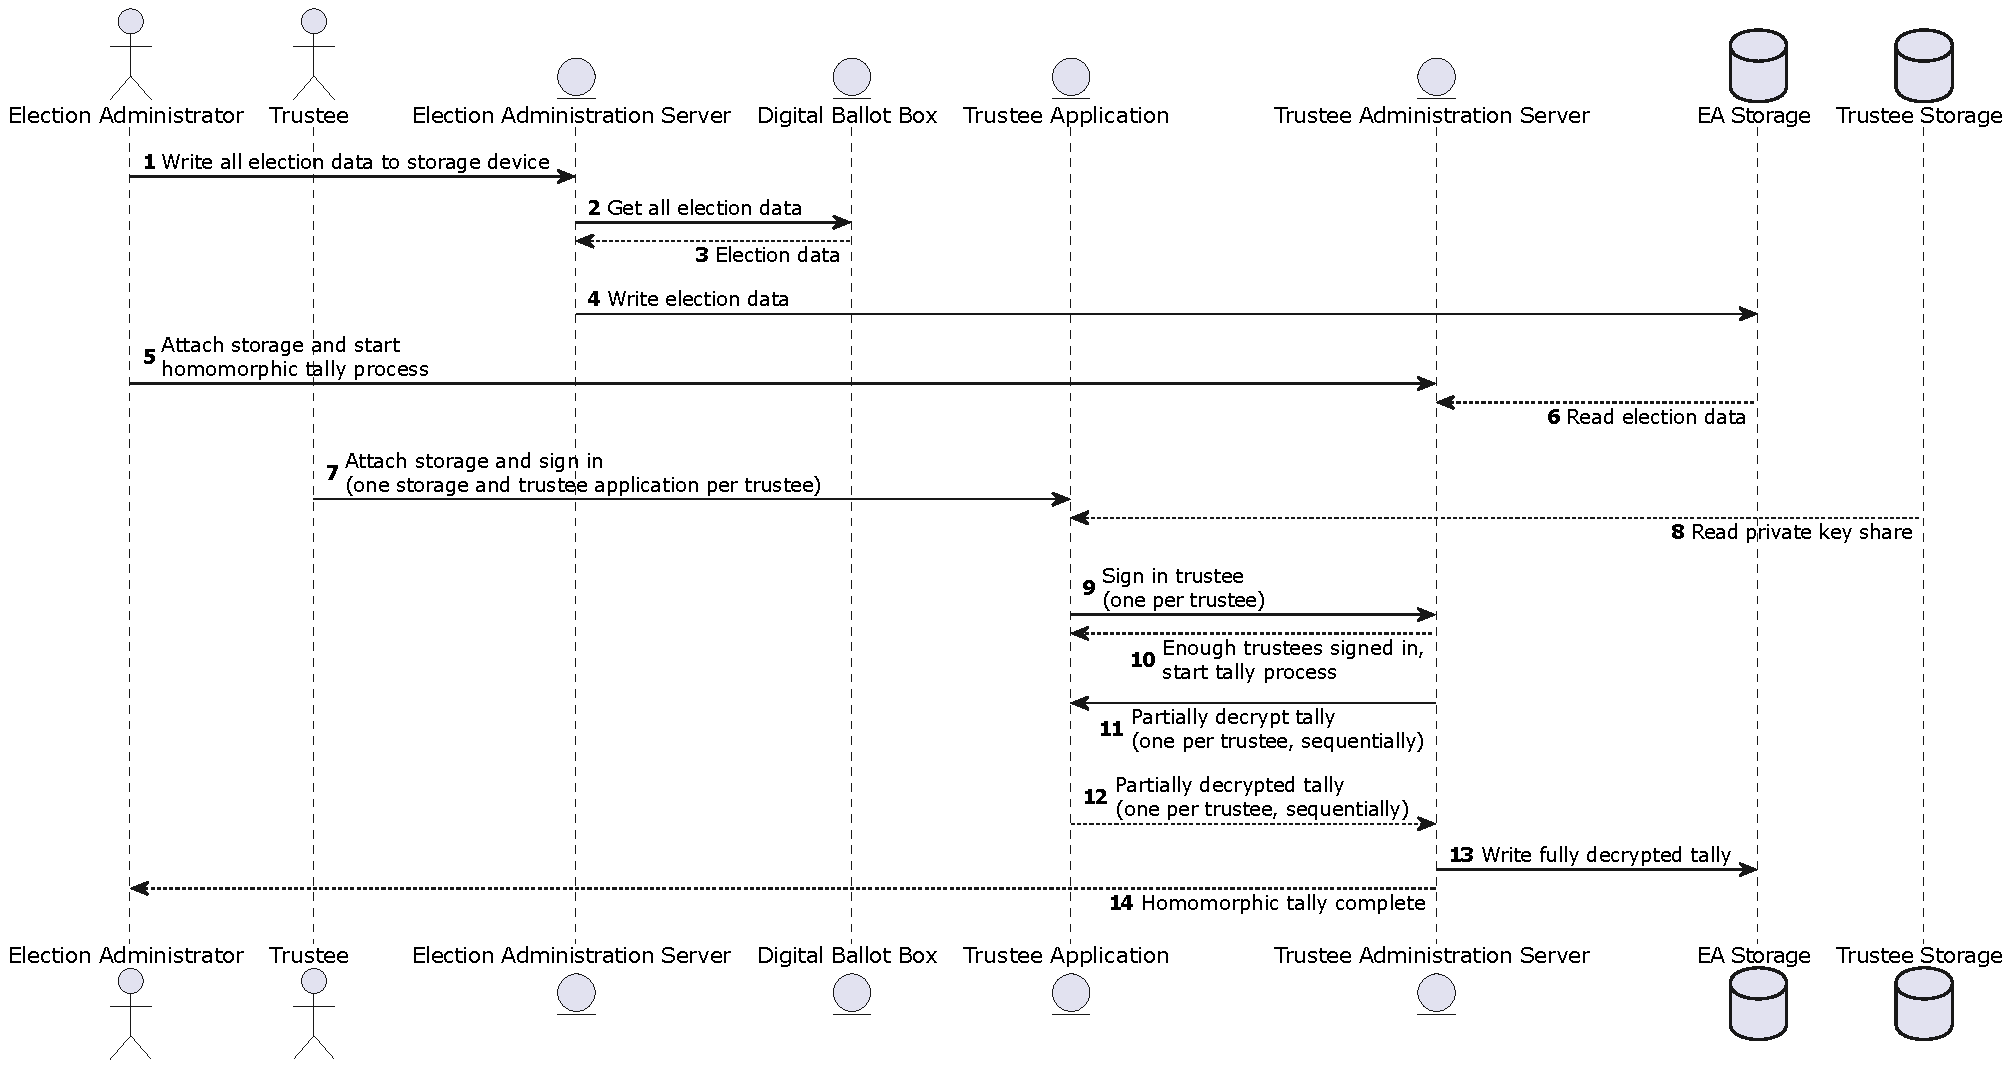
\includegraphics[width=\textwidth]{diagrams/seq-homomorphic-tally.pdf}

Having provided informal overviews of all the protocol interactions within the system, we will next describe threats to the system and, where applicable, our mitigations of those threats. More details about the protocol are available in our systems architecture specification, which includes precise descriptions of the system's principals, events, channels, messages, and use cases, and in our formal protocol specification, which includes precise descriptions of the entire protocol and its correctness and security properties.

\pagebreak
\section{Threats, Attacks, and Mitigations}

As many subsystems of the E2E-VIV system are connected to the Internet, it is subject to the same wide range of ``standard'' (sometimes quite serious) threats arising from Internet connectivity as any other Internet-connected system. Techniques for mitigating such threats are generally well-known, and we will not, in most cases, discuss those threats in detail here. As discussed earlier, general cybersecurity practices that address such threats are modeled as black boxes under the \hyperlink{M8}{M8 (Cybersecurity---Escalation)}, \hyperlink{M9}{M9 (Cybersecurity---Intrusion)}, \hyperlink{M10}{M10 (Cybersecurity---Malware)}, \hyperlink{M11}{M11 (Cybersecurity---Supply chains)}, and \hyperlink{M12}{M12 (Cybersecurity---Virtualization)} mitigations.

Some of those threats are widely recognized as unmitigatable with today's commodity Internet technology in the face of the most powerful adversaries, such as major nation states' intelligence agencies. In particular, there are several critical inherent weaknesses present in \emph{any} deployed distributed system that uses (1)~the public Internet for communication, (2)~consumer electronic devices as endpoints, or (3)~poorly certified/evaluated proprietary commercial technology such as today's commercial voting systems, printers, or network equipment.

Large-scale or highly-targeted \emph{distributed denial of service (DDoS) attacks} are very difficult to mitigate except by the largest companies. \emph{On-device malware} on consumer devices such as smart phones, developer workstations, and deployed on-premises or cloud-based servers is very difficult to reliably prevent, detect, and mitigate. Systems that mitigate \emph{network attacks} are very difficult to deploy and operate, and \emph{compromises inserted into the hardware, firmware, or software supply chain of a system} by advanced adversaries are very difficult to detect and mitigate.

In addition to these Internet-related threats, the E2E-VIV system is also subject to threats specific to voting systems and the cryptographic protocols and primitives used for constructing them. Given the nature of the E2E-VIV system and its possible deployments, we start from the following assumptions:

\begin{enumerate}

    \item The E2E-VIV system will be a target for advanced persistent threat actors (APTs) such as nation-states.

    \item Such APTs can acquire access to all trust zones in the system, including the \textbf{Air-Gapped Network} (e.g., by corrupting a \textbf{Trustee} or \textbf{Election Administrator}, or performing a supply-chain attack on equipment used for the \textbf{Trustee Administration Server} or \textbf{Trustee Application}).

    \item Such APTs will have full knowledge of the E2E-VIV system, including all source code, binaries, protocol specifications, evidence of correctness and security, etc.

\end{enumerate}

\subsection{E-voting Properties}

To derive attacks specific to E2E-VIV systems, it is useful to recall the properties that secure voting systems are expected to have. Adversaries will seek to violate or undermine these properties. The following table lists these properties together with a broad classification into the three security objectives of the CIA triad (\textbf{C}onfidentiality, \textbf{I}ntegrity, \textbf{A}vailability) as well as the threat types referred to in STRIDE (\textbf{S}poofing, \textbf{T}ampering, \textbf{R}epudiation,\footnote{\label{footnote:repudiation} ``Repudiation,'' as a STRIDE threat, covers both situations when we want to be able to repudiate something and situations when we want to not be able to repudiate something. Sometimes, we effectively want the voter to not be able to say they did something (essentially the opposite of repudiation), but for STRIDE purposes we still classify that under ``Repudiation.''}  \textbf{I}nformation disclosure, \textbf{D}enial of service, and \textbf{E}scalation of privilege)~\cite{MicrosoftSecuritySTRIDEChart2007,GroeneveldMasteringSTRIDE}. Items not marked explicitly with a reference are taken from Sampigethaya and Poovendran \cite{SampigethayaPoovendranFrameworkTaxonomy2006}, Cetinkaya \cite{CetinkayaAnalysisSecurity2008}, or a combination thereof.

\begin{longtblr}{colspec={||Q[m,wd=0.8in]|Q[m,wd=3.4in]|Q[m]|Q[m]||}, rowhead=1, cells={font=\fontsize{9pt}{10pt}\selectfont}}

\hline

\textbf{E-voting Property} & \textbf{Description} & \textbf {CIA Triad} & \textbf{STRIDE} \\
\hline

Accuracy &
{ The votes must be correctly recorded and tallied. \\ Votes cast by invalid voters must not be included in the tally. \\ Cast votes cannot be altered, deleted, invalidated or copied. } & Integrity &
{ Spoofing, \\ Tampering } \\
\hline

Privacy &
A voter and their vote cannot be linked. &
Confidentiality &
{ Information \\ disclosure } \\
\hline

Eligibility &
Only valid voters who meet certain predetermined criteria are eligible to vote. &
Integrity &
Spoofing \\
\hline

{E2E \\ Verifiability \\ (E2E-V)} \cite{BenalohEtAlEndtoendVerifiability2015} &
{ Voters can get convincing evidence that their encrypted votes accurately reflect their choices. \\ Voters or their designees can check that their encrypted votes have been correctly included in the tally. \\ Any member of the public can check that all the published encrypted votes are correctly included in the tally. } &
Integrity &
Tampering \\
\hline

{Eligibility \\ Verifiability} \cite{KremerEtAlElectionVerifiability2010} &
Anyone can check that each vote in the election outcome was cast by a registered voter, and at most one vote is counted per voter. &
Integrity &
{ Spoofing, \\ Tampering }\\
\hline

Receipt-freeness \cite{DelauneEtAlCoercionresistanceReceiptfreeness2006} &
A voter does not gain any information (a ``receipt'') that can be used to prove to anyone else that they voted in a certain way. &
Confidentiality &
Repudiation \\
\hline

{Coercion \\ Resistance} \cite{DelauneEtAlCoercionresistanceReceiptfreeness2006} &
A voter cannot cooperate with a coercer to prove to them that they voted in a certain way. & Confidentiality &
Repudiation \\
\hline

{Everlasting \\ Privacy} \cite{HainesEtAlSoKSecure2023} &
Even computationally unbounded adversaries cannot violate the Privacy property for any past election. &
Confidentiality &
{Information \\ disclosure} \\
\hline

Fairness &
No one can compute a partial tally before the election concludes. &
Integrity &
{Information \\ disclosure} \\
\hline

$D$-Dispute-freeness &
A mechanism is provided to resolve disputes in some dispute set $D$. &
Integrity &
Repudiation \\
\hline

Robustness &
The system is resilient to attacks and faults that can interrupt or prevent its normal operation. &
Availability &
{Denial of \\ service} \\
\hline

Scalability &
The system can scale to large numbers of voters without degrading performance or the user experience. &
Availability &
{Denial of \\ service} \\
\hline

\end{longtblr}

We derive concrete security objectives from these properties and group them into the three main categories of the CIA triad. In this derivation, we use abbreviations to denote specific entities (subsystems, actors, assets) within the system; these are defined in \autoref{appendix:abbreviations}.

\subsection{Security Objective: Integrity}

The e-voting properties of Accuracy, Eligibility, Fairness, Verifiability, and Dispute-freeness are mapped to this security objective.

\subsubsection{Correctness (Accuracy + Eligibility + Fairness)}

\input{db/correctness_tree}

The following table\footnote{This and subsequent tables are generated automatically from the semi-formal threat model. They represent \emph{static views} into the overall threat model, which continues to evolve as we refine the protocol.} lists the attacks against correctness properties and their mitigations. Note that the numbering of attacks and mitigations in this and subsequent security objective-centered attack/mitigation tables matches the numbering in the \emph{complete} attack table (\autoref{appendix:attacks}) and mitigation table (\autoref{appendix:mitigations}), and some attack and mitigation numbers are therefore skipped. Note also that some attacks in these tables (e.g., \hyperlink{ATK27}{ATK27.~Premature tabulation}) do not have their own specific mitigations, but are instances of more general \emph{abstract} attacks (described in \autoref{sec:abstract-attacks}); in such cases the table refers to more general mitigations for the abstract attacks.

Various tools and techniques enable rigorous analysis of attacks and their inter-dependencies, particularly attack trees and attack graphs~\cite{BruceSchneierAttackTrees1999,KonstaSurveyAutomaticGeneration2023,NguyenAutomatedAttack2020}. We have not used these concepts or tools in this analysis, as they are more appropriately applied to the design of a full system rather than a single component like a cryptographic protocol or library.

\input{db/c_attack_mitigation_table}

\subsubsection{Verifiability}

Verifiability refers to the ability to verify that the correctness requirements defined above hold. Verifiability confers a degree of \emph{software independence}~\cite{RivestVirzaSoftwareIndependence2016}, insofar as deviations from correct execution can be detected. The degree to which this is achieved is usually limited for E2E-VIV systems because they employ software to carry out verification itself. This limitation can be somewhat\footnote{The meaning of ``somewhat'' varies considerably based upon the decisions made about design and formal methods use when creating and assuring a specific system. Douglas Wikstr\"{o}m's book, upon which our cryptographic analysis is based, delves into this topic in depth from the point of view of tight analyses of threats to cryptographic security.} ameliorated through the use of multiple independent Verifier Application (VER) implementations, as well as the use of formal verification tools to create a formal assurance case for a system's implementation.

Note also that although Verifiability and Correctness are related, they may vary independently. It is possible for a system to exhibit all four possible binary combinations of the two ($V\wedge C$, $V\wedge\neg C$, $\neg V\wedge C$, $\neg V\wedge \neg C$), just as it is possible for an adversary to perform attacks on either one. A system satisfying Integrity must satisfy all three sub-goals, including Correctness and Verifiability.

\input{db/verifiability_tree}

\input{db/v_attack_mitigation_table}

\paragraph{Interpretation of verifiability}

Verifiability is interpreted as a double implication. A condition is verifiable when \emph{a verification operation reports failure if and only if the condition is false}. Using attack \hyperlink{ATK24.2}{24.2} as an example, we have that ``The checking application does not provide correct information about audited cryptograms.'' expands to:
%
\begin{itemize}
    \item The checking application reports success for an invalid cryptogram and/or
    \item The checking application reports failure for a valid cryptogram.
\end{itemize}

It is also possible to interpret verifiability as a weaker single implication: \emph{A verification operation reports failure if the condition is false.}
%
If the condition is true, the verification operation may report failure or success. This is closer to the notion of software independence, which requires that failed conditions cannot go undetected. But this interpretation would imply that a verification implementation that always returns failure would satisfy the verifiability property in a trivial way.

\hypertarget{further-remarks-checking-application}{\paragraph{Further remarks on the checking application}}
There are several checks that can be performed by voters or any other observer. At a minimum, the Ballot Check Application (BCA) implements the cast-as-intended verification which ensures that ballot cryptograms correspond to voter intent. But the BCA could also implement the recorded-as-cast, counted-as-recorded, and eligibility verifications. The last two are also performed by the Verifier Application.

\paragraph{Further remarks on eligibility verifiability}

In the current model, the EA is responsible for defining eligibility as well as operating the authentication and authorization mechanisms that conform to said eligibility. The following tasks must be performed by the EA:

\begin{itemize}
    \item Define the set of eligible voters
    \item Produce signatures on eligible voter certificates (whose private keys sign ballots)
    \item Produce credentials with which eligible voters will authenticate
    \item Operating the systems responsible for authentication and authorization
\end{itemize}

It is also possible to split these two responsibilities such that one party defines eligibility (for example, a separate Census Authority) and the other operates the systems that enforce it. This is one instance of the \hyperlink{M28}{M28 Trust distribution} mitigation that protects against eligibility stuffing.

\paragraph{Further remarks on M7, M24, M27, and cryptogram linking}

\hyperlink{M27}{M27 (Tamper evident bulletin board)} has been defined as a mitigation against attacks on verifiability. However, M27 also has the effect of extending the reach of \hyperlink{M24}{M24 (Recorded as cast verifiability)} verifications into \hyperlink{M7}{M7 (Counted as recorded verifiability)}. M27 links cryptograms cast by different voters in a way that couples their verification outcomes. If a voter performs an M24 verification that is linked with a cryptogram that is the subject of an M7 verification, the latter will indirectly provide M7 for the former cryptogram. The condition necessary for this coupling is some degree of overlap of verification intervals that the adversary must account for when performing attacks.

\subsubsection{Dispute-freeness}

Following Basin et al.\cite{BasinEtAlDisputeResolution2020}, we define the dispute set $D$ as
%
\input{db/d1_d2_tree}

Note that, though we refer to them in attack and mitigation tables as security objectives, these are not security objectives in the same sense as the other security objectives we have discussed so far; rather, each $Di$ should be thought of as generating security objectives of the form ``the dispute described in $Di$ can always be resolved.''

\input{db/d1_d2_attack_mitigation_table}

If we augment the dispute set $D$ to $D^*$ by adding the following:
%
\input{db/d3_tree}

Then, if the system does not satisfy $D^*$-Dispute-freeness, and the election is protected against malicious voting applications by invalidating its outcome when a sufficient number of voters make reports, the following attack on availability becomes possible.

\input{db/d3_attack_mitigation_table}

\subsection{Security Objective: Confidentiality}

The e-voting properties of Privacy, Everlasting Privacy, Receipt-freeness, and Coercion-resistance are mapped to this security objective.

\input{db/confidentiality_tree}

\input{db/p_attack_mitigation_table}

\subsection{Security Objective: Availability}

The e-voting properties of Robustness and Scalability are mapped to this security objective.

\input{db/availability_tree}

\input{db/a_attack_mitigation_table}

\subsection{``Abstract'' Attacks}
\label{sec:abstract-attacks}

In the above sections the details of some attacks have been omitted for clarity; we call these \emph{abstract} attacks. They include attacks related to compromised devices, compromised networks, broken cryptography, phishing, spoofing, side channels, and generalized ``corruption.'' \emph{Concrete} attacks (like those described above) can be instantiations of these abstract attacks. For example, \hyperlink{ATK1.3}{ATK1.3 Compromised Device (TAS)} is a concrete attack that involves compromising the \textbf{Trustee Administration Server}, and is thus an instantiation of abstract attack \hyperlink{AATK2}{AATK2 Compromised Device}. It is not decomposed further into the various ways that the TAS can be compromised, and general mitigations against device compromise are not listed with it. In the following table, we list all the abstract attacks, their decompositions, and their general mitigations.

\input{db/abstract_attack_table}

\appendix

\pagebreak
\section{Abbreviations}
\label{appendix:abbreviations}

The following table lists the abbreviations used throughout this document to refer to system entities, along with the entities to which they refer and each entity's type.

\input{db/context_table}

\pagebreak
\section{Concrete Attack Table}
\label{appendix:attacks}

The following table lists all concrete attacks and their corresponding security objectives. Each of these attacks is listed along with its individual mitigations in the appropriate earlier section of the document; this listing is intended as a reference that gathers all the attacks in numerical order and links them to their corresponding security objectives.

\input{db/all_attack_table}

\pagebreak
\section{Mitigation Table}
\label{appendix:mitigations}

The following table lists all mitigations and the attacks they mitigate. Each of these mitigations is referenced in an earlier section of the document; this listing is intended as a reference that gathers all the mitigations in numerical order and links them to the abstract and concrete attacks they mitigate.

\input{db/mitigation_table}

\pagebreak
\printbibliography[heading=bibintoc]

\end{document}
